\documentclass[tikz]{standalone}
\usepackage{pgfplots}
\pgfplotsset{compat=1.15}
\usepackage{mathrsfs}
\usetikzlibrary{arrows,calc}
\usepackage{tkz-euclide}

\pagestyle{empty}

\definecolor{AngleClr}{rgb}{0,0.39215686274509803,0}
\definecolor{ShapeClr}{rgb}{0.6,0.2,0}

\begin{document}

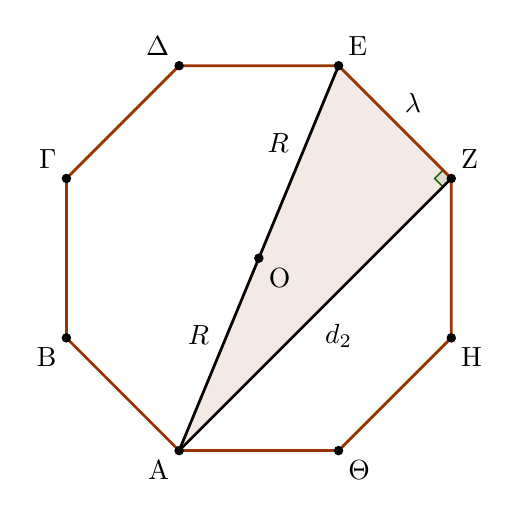
\begin{tikzpicture}[scale=.75]
\tkzSetUpLine[line width=1pt,color=black]
\tkzSetUpPoint[fill=black]

\tkzDefPoints{0/0/P0,2.7/0/P1}

\tkzDefRegPolygon[side,sides=8](P0,P1)

\tkzDefMidPoint(P1,P2) \tkzGetPoint{M1}
\tkzDefMidPoint(P2,P3) \tkzGetPoint{M2}
\tkzDefMidPoint(P3,P4) \tkzGetPoint{M3}
\tkzDefMidPoint(P4,P5) \tkzGetPoint{M4}
\tkzDefMidPoint(P5,P6) \tkzGetPoint{M5}
\tkzDefMidPoint(P6,P7) \tkzGetPoint{M6}
\tkzDefMidPoint(P7,P8) \tkzGetPoint{M7}
\tkzDefMidPoint(P8,P1) \tkzGetPoint{M8}


\tkzFillPolygon[fill=white](P1,P2,P3,P4,P5,P6,P7,P8)

\tkzDefCircle[circum](P1,P2,P3) \tkzGetPoint{O}
% \tkzDrawCircle[line width=0.7pt,black](O,P1)

\tkzMarkRightAngles[line width=0.5pt, size=.2,color=AngleClr,fill=AngleClr,fill opacity=0.1](P1,P4,P5)

\tkzDrawSegments[line width=1pt](P1,P4 P1,P5)

\tkzDrawPolygon[color=ShapeClr](P1,P2,P3,P4,P5,P6,P7,P8)

\tkzFillPolygon[fill=ShapeClr,fill opacity=0.1](P1,P4,P5)

\tkzDrawPoints[size=3](O,P1,P2,P3,P4,P5,P6,P7,P8)
\tkzLabelPoint[below left](P1){$\rm A$}
\tkzLabelPoint[below right](P2){$\rm \Theta$}
\tkzLabelPoint[below right](P3){$\rm H$}
\tkzLabelPoint[above right](P4){$\rm Z$}
\tkzLabelPoint[above right](P5){$\rm E$}
\tkzLabelPoint[above left](P6){$\rm \Delta$}
\tkzLabelPoint[above left](P7){$\rm \Gamma$}
\tkzLabelPoint[below left](P8){$\rm B$}

\tkzLabelPoint[below right](O){$\rm O$}
\tkzLabelSegment[below right](P1,P4){$d_2$}
\tkzLabelSegment[above right](P4,P5){$\lambda$}

\tkzLabelSegment[above left](P1,O){$R$}
\tkzLabelSegment[above left](O,P5){$R$}

\end{tikzpicture}

\end{document}
